\documentclass{article}
\usepackage{graphicx}
\usepackage{amsmath}
\usepackage{amssymb}
\usepackage{enumitem}
\usepackage{hyperref}

\begin{document}
\title{Lista de Exercícios 3 - Cálculo 2}
\author{Débora D'Angelo Reina de Araujo}
\date{\today}

\maketitle

\begin{enumerate}
    \item Resolver em ambiente computacional o exercício 1 da seção 8.3 (pág. 276) do livro do Apostol de Cálculo 2. Explore os recursos de plot da ferramenta computacional escolhida por você para exibir as curvas e superfícies de nível.
    
    \begin{enumerate}[label=1.\arabic*.]
        \item Seja $f$ um campo escalar definido num conjunto $S$ e $c$ um número real dado. 
        O conjunto de todos os pontos x de $S$ tais que $f(x) = c$ é chama-se um conjunto de nível de $f$. 
        (Problemas de natureza geométrica e física tratando com conjunto de nível serão analisados neste capítulo.) 
        Para cada um dos seguintes campos escalates, $S$ é todo o espaço $\mathbb{R}^{n}$. 
        Fazer o desenho relativo aos conjuntos de nível correspondendo aos valores de $c$ dados.

        \begin{enumerate}[label=(\alph*)]
            \item $f(x, y) = x^2 + y^2, \hspace{1cm} c = 0, 1, 4, 9.$
            \begin{figure}[!ht]
                \centering 
                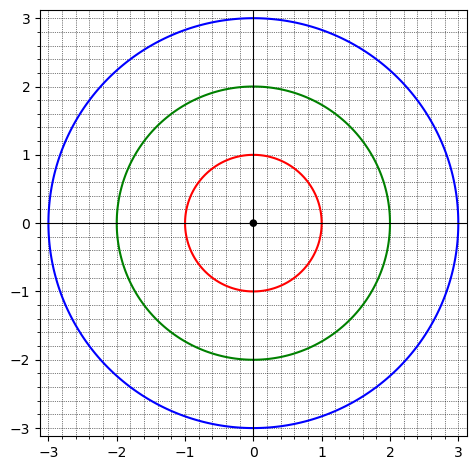
\includegraphics[width=0.7\linewidth]{nivel1.png} 
                \label{fig:imagem1}
            \end{figure} \\
            \item $f(x, y) = e^{xy}, \hspace{1cm} c = e^{-2}, e^{-1}, 1, e, e^2, e^3.$
            \begin{figure}[!ht]
                \centering 
                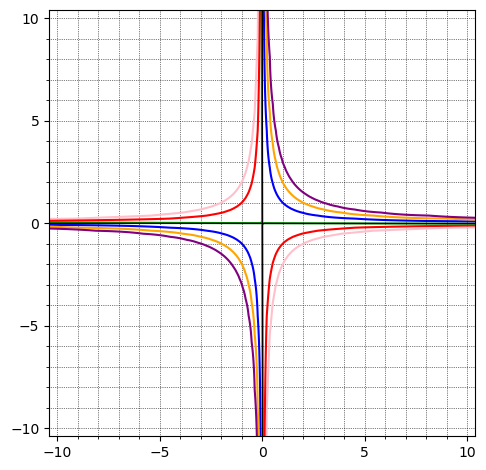
\includegraphics[width=0.7\linewidth]{nivel2.png} 
                \label{fig:imagem1}
            \end{figure}
            \item $f(x, y) = cos(x+y), \hspace{1cm} c = -1, 0, \frac{1}{2}, \frac{\sqrt{2}}{2}, 1.$
            \begin{figure}[!ht]
                \centering 
                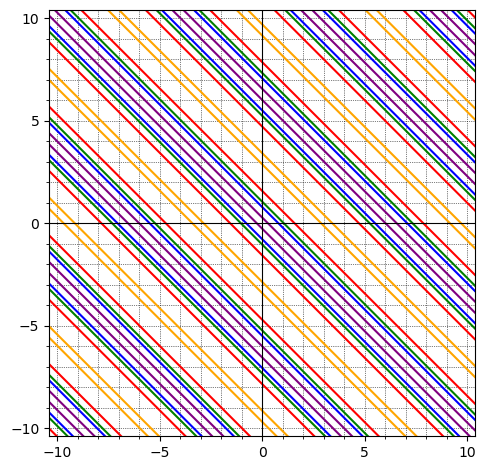
\includegraphics[width=0.7\linewidth]{nivel3.png} 
                \label{fig:imagem1}
            \end{figure} \\
            \item $f(x, y, z) = x + y + z, \hspace{1cm} c = -1, 0, 1.$
            \begin{figure}[!ht]
                \centering 
                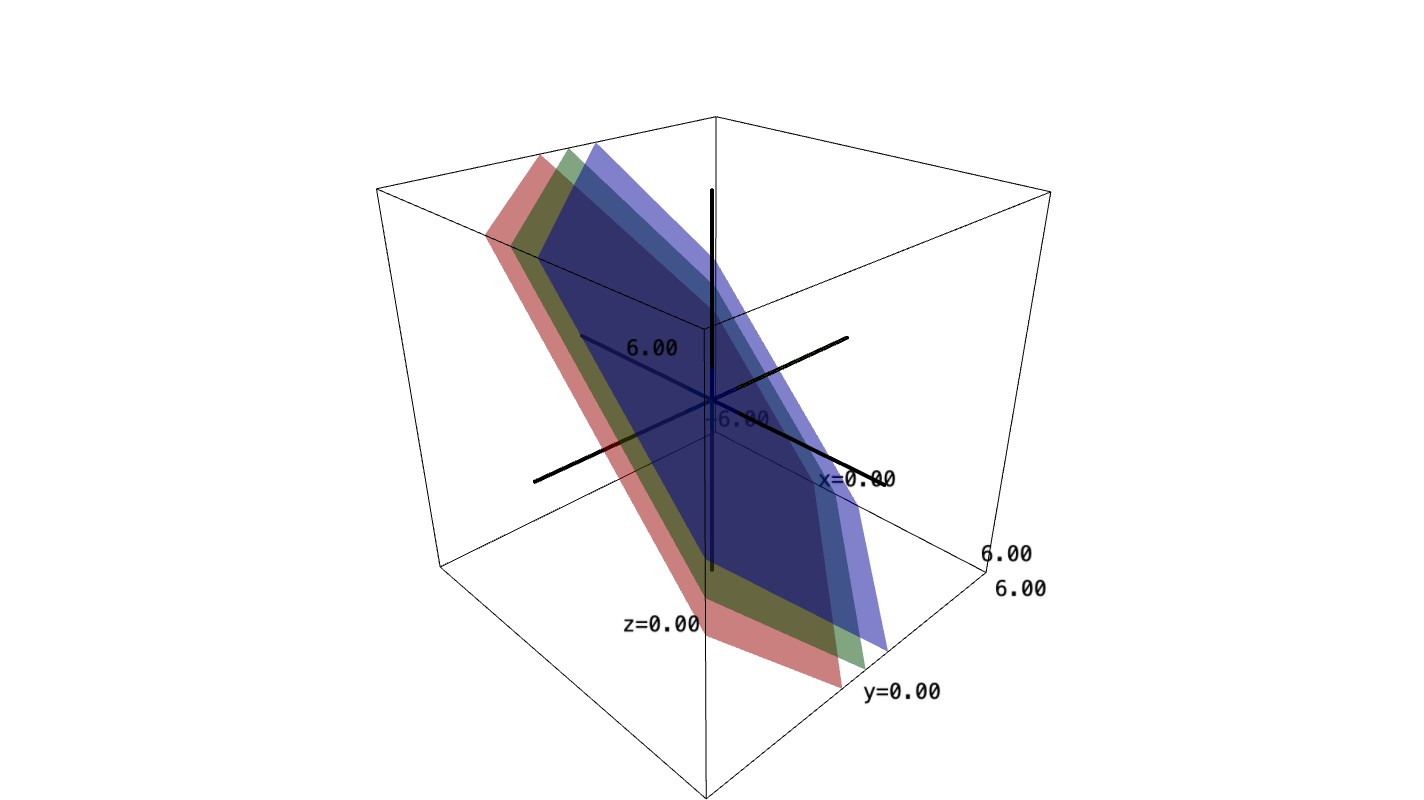
\includegraphics[width=0.7\linewidth]{nivel4.png} 
                \label{fig:imagem1}
            \end{figure}
            \item $f(x, y, z) = x^2 + 2y^2 + 3z^2, \hspace{1cm} c = 0, 6, 12.$
            \begin{figure}[!ht]
                \centering 
                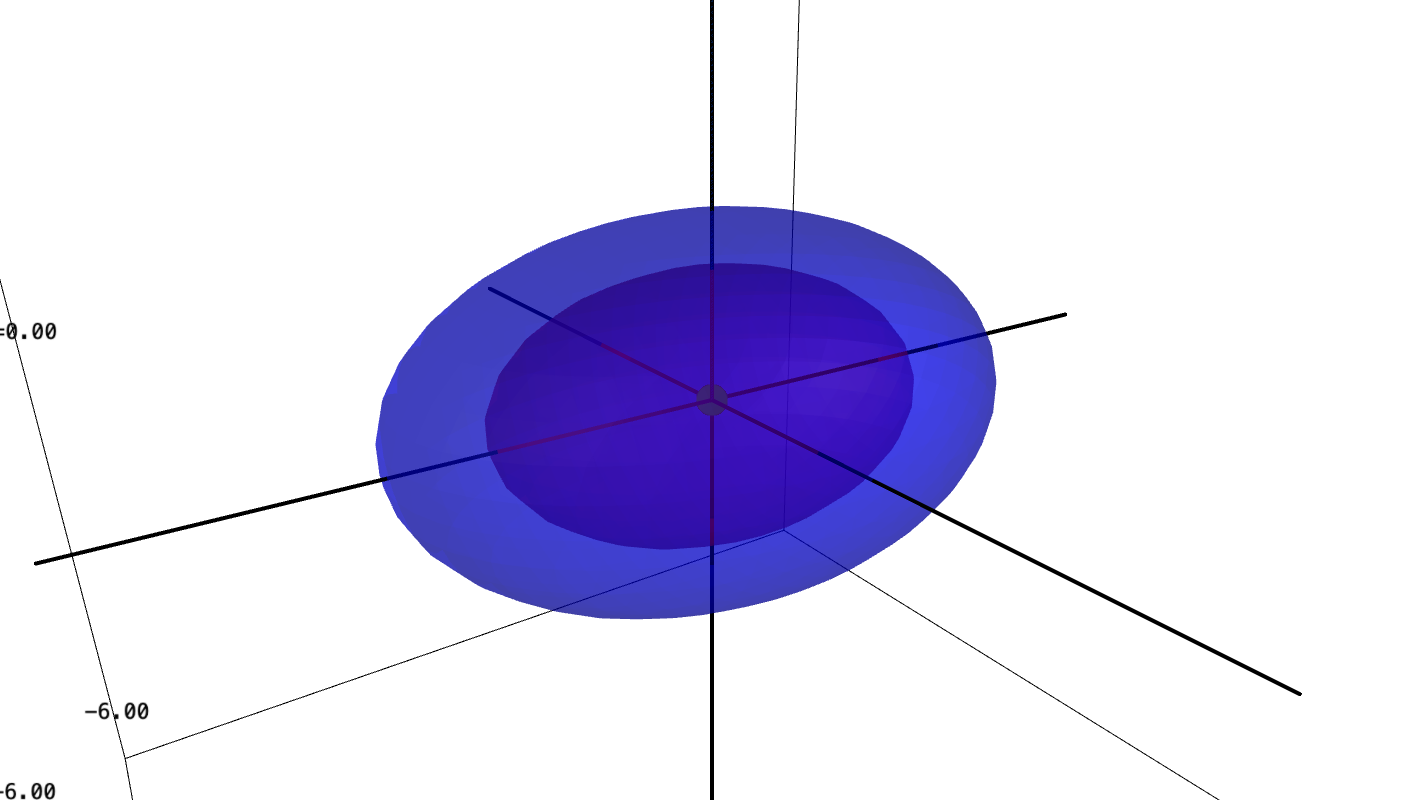
\includegraphics[width=0.7\linewidth]{nivel5.png} 
                \label{fig:imagem1}
            \end{figure}
            \item $f(x, y, z) = sen(x^2 + y^2 + z^2), \hspace{1cm} c = -1, -\frac{1}{2}, 0, \frac{\sqrt{2}}{2}, 1$
            \begin{figure}[!ht]
                \centering 
                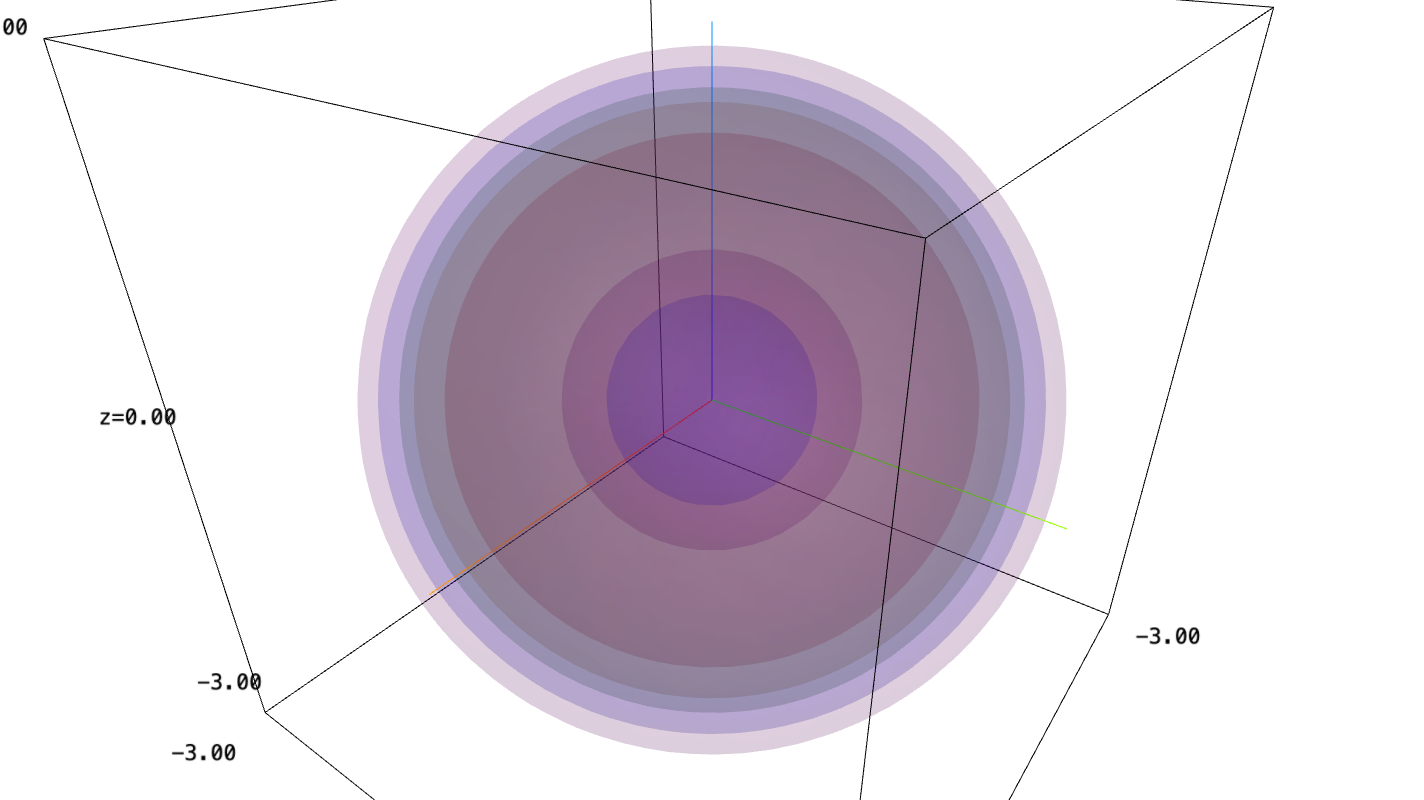
\includegraphics[width=0.7\linewidth]{nivel6.png} 
                \label{fig:imagem1}
            \end{figure}
        \end{enumerate}
    \end{enumerate}
    \item Desenhe em ambiente computacional as seguintes figuras, marque um ponto sobre elas e trace uma curva sobre a sua superfície.
    \begin{itemize}
        \item Paraboloide elítico: $S = \{(x, y, z) \in \mathbb{R}^3 | z = \frac{x^2}{a^2} + \frac{y^2}{b^2}\}$
        \item Paraboloide hiperbólico: $S = \{(x, y, z) \in \mathbb{R}^3 | z = \frac{x^2}{a^2} - \frac{y^2}{b^2}\}$
    \end{itemize}
    Escolha a sua descrição preferida para as superfícies (campos vetoriais), implícita ou paramétrica e justifique a sua resposta.
    \begin{figure}[!ht]
        \centering
        \begin{subfigure}{\textwidth} 
            \centering
            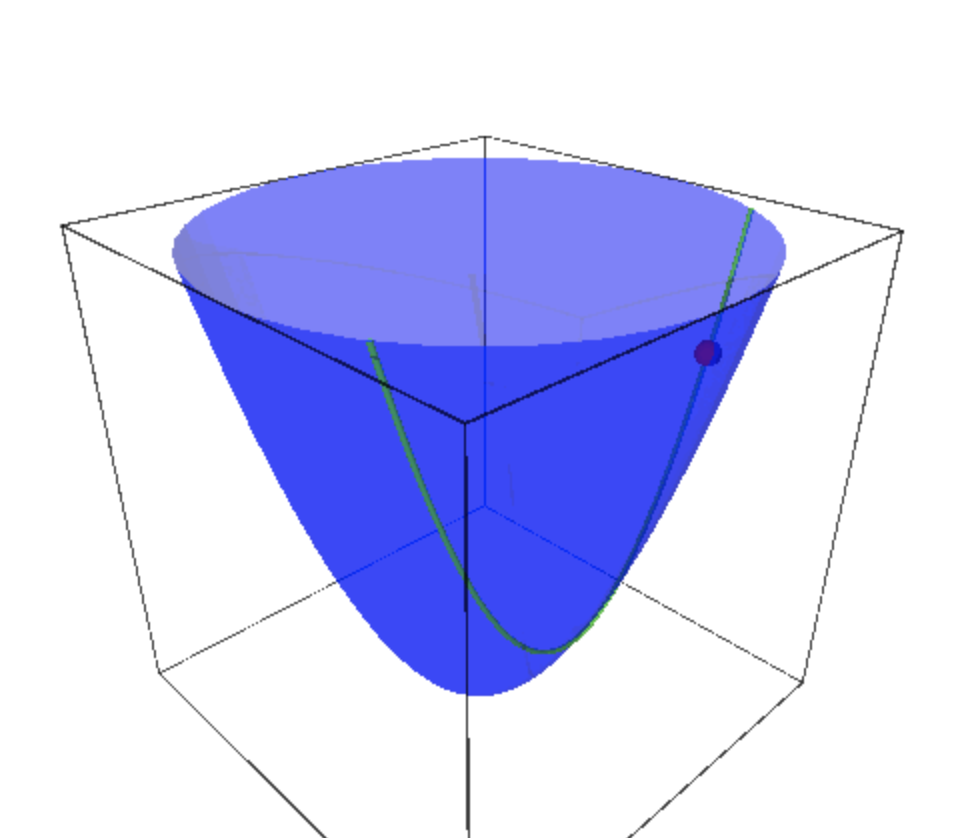
\includegraphics[width=0.3\linewidth]{anim1.png} 
            \label{fig:imagem1}
        \end{subfigure}
        \begin{subfigure}{\textwidth} 
            \centering
            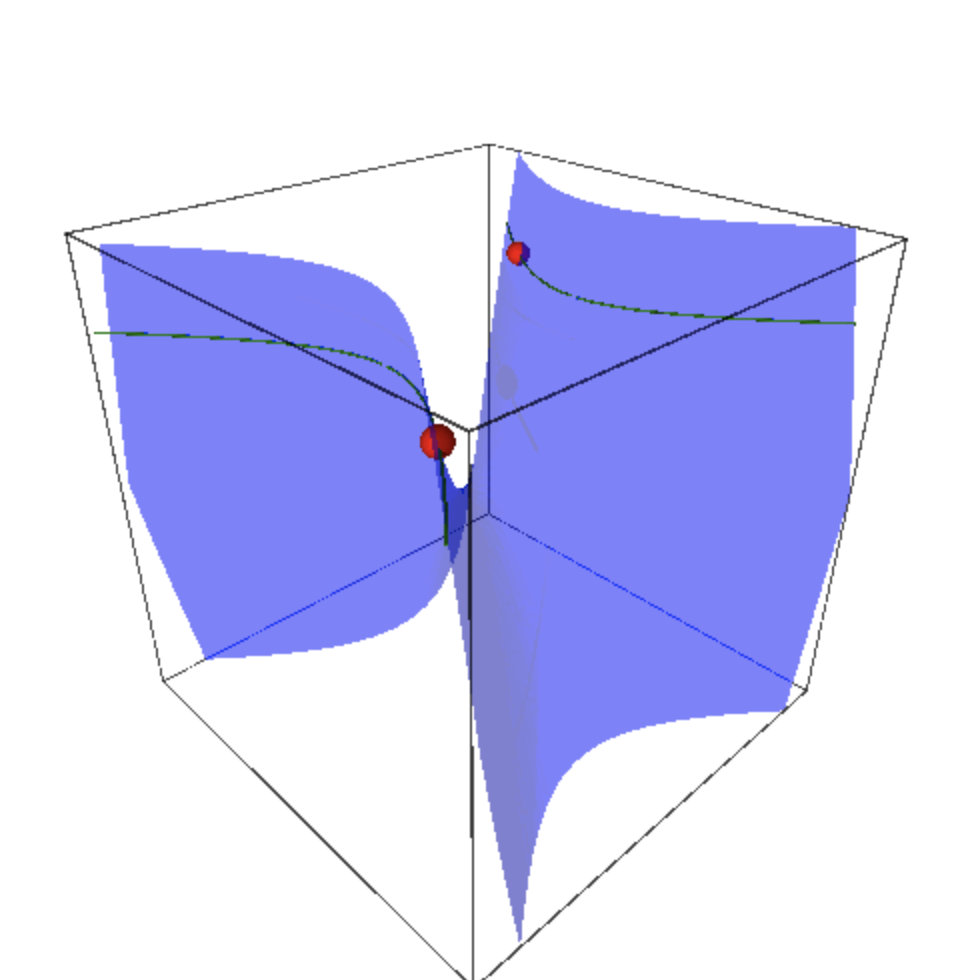
\includegraphics[width=0.3\linewidth]{anim2.png} 
            \label{fig:imagem2}
        \end{subfigure}
        \label{fig:exemplo_duas_imagens} 
    \end{figure} \\
    Para desenhar a superfície é melhor a descrição implícita, pois a equação já esta dada. Já para traçar uma curva sobre ela, é melhor a paramétrica, pois podemos escolher um parâmetro e traçar a curva em função dele.\\
    É perceptível que as animações feitas a partir de uma curva paramétrica são mais eficiêntes de serem computadas e possuem animação mais suave.\\
    \item Desenhe duas ou mais opções de superfícies de rotação que te pareçam interessantes. \\ 
    Superfícies de rotação emergem da rotação de uma curva geratriz em torno de um eixo. Considere uma curva plana continha no plano $\Pi_{xz}$ da forma $\alpha(u) = (f(u), 0, g(u)), u \in I \subset \mathbb{R}$ e produza a rotação em torno do eixo vertical variando o parametro $v$ da seguinte forma $$X(u, v) = (f(u)cos(v), f(u)sin(v), g(u))$$ Produza uma animação da curva geratriz com a variação do parâmetro.
    \begin{figure}[!ht]
        \centering
        \begin{subfigure}{\textwidth} 
            \centering
            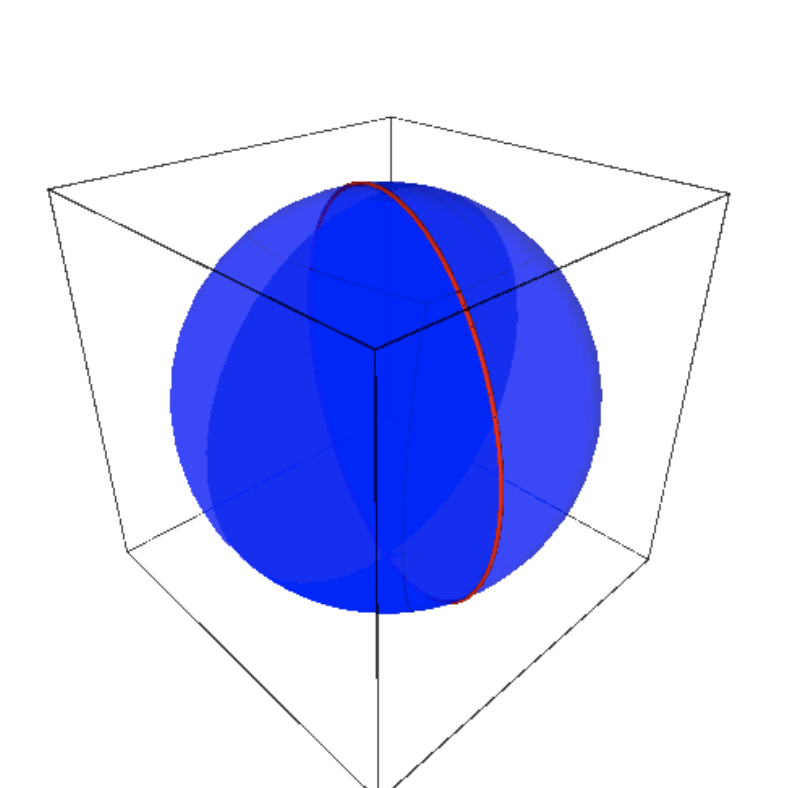
\includegraphics[width=0.3\linewidth]{anim3.png} 
            \label{fig:imagem1}
        \end{subfigure}
        \begin{subfigure}{\textwidth} 
            \centering
            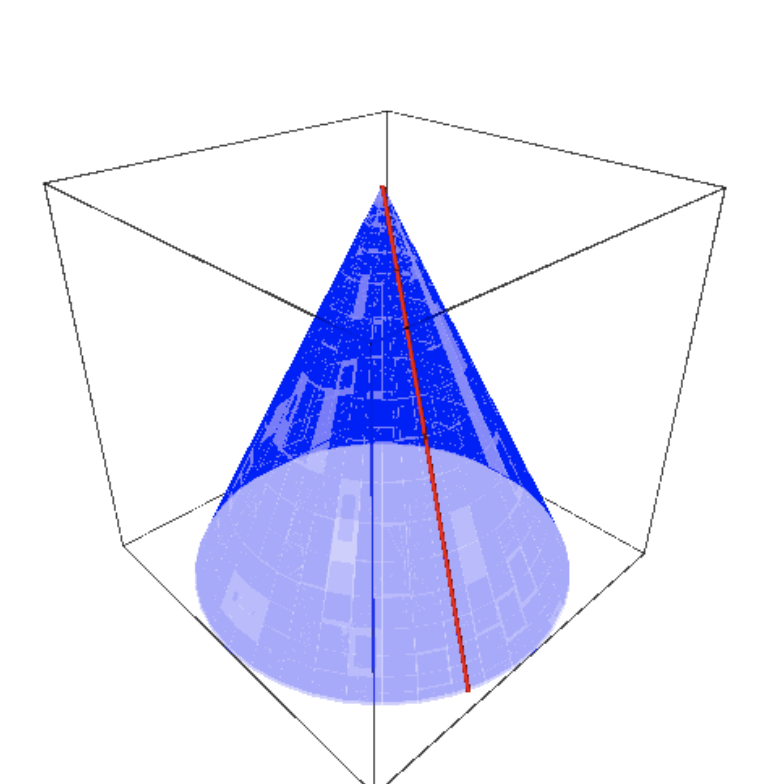
\includegraphics[width=0.3\linewidth]{anim4.png} 
            \label{fig:imagem2}
        \end{subfigure}
        \label{fig:exemplo_duas_imagens} 
    \end{figure} \\
    Superfícies rotacionadas a partir de, respectivamente: 
    $$\alpha(t) = (cos(t), 0, sin(t))$$
    $$\beta(t) = (cos^{2}(t), 0, sin^{2}(t))$$
    \item Escolha um conceito de física para representar computacionalmente como campo vetorial.
    \begin{figure}[!ht]
        \centering
        \begin{subfigure}{\textwidth} 
            \centering
            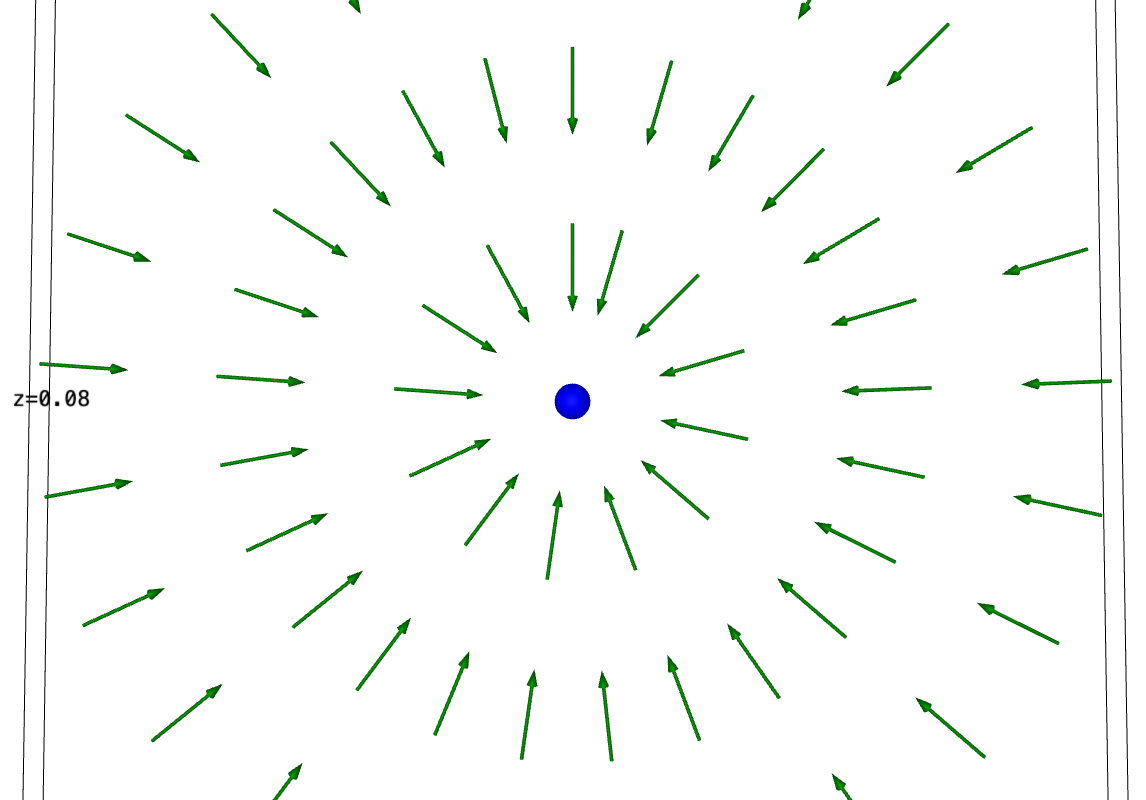
\includegraphics[width=0.3\linewidth]{tensorfield1.png} 
            \label{fig:imagem1}
        \end{subfigure}
        \begin{subfigure}{\textwidth} 
            \centering
            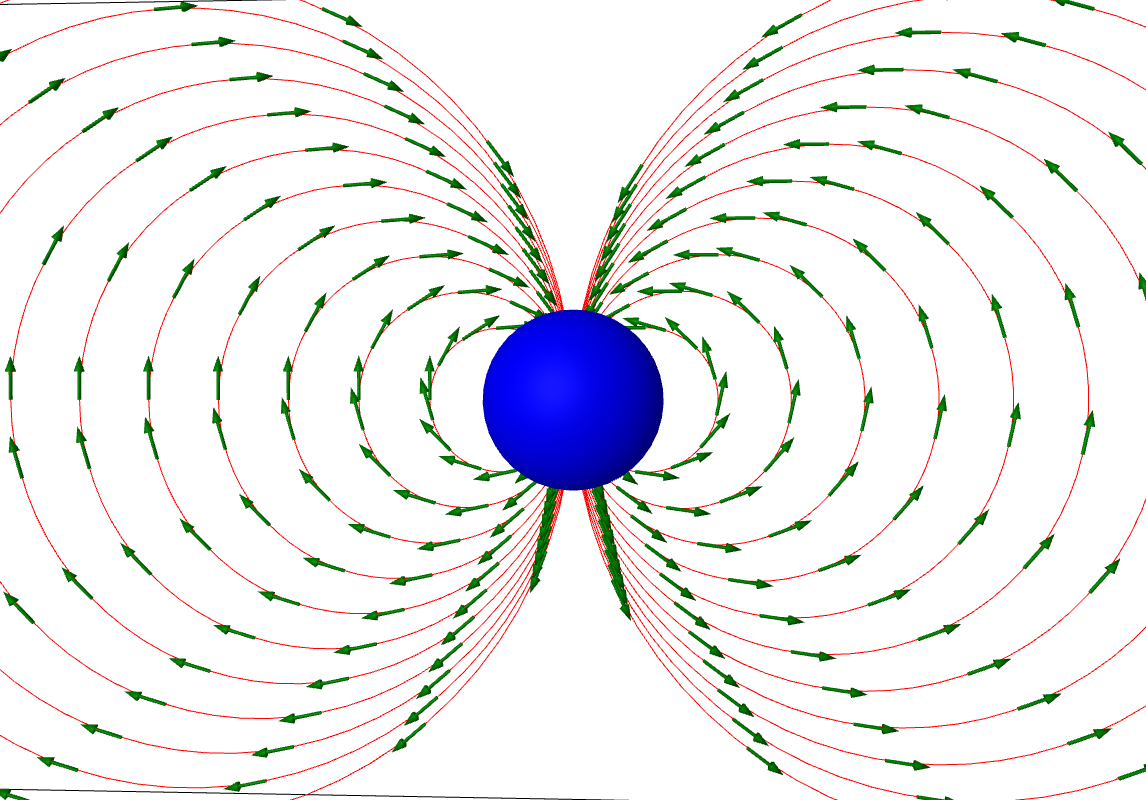
\includegraphics[width=0.3\linewidth]{tensorfield2.png} 
            \label{fig:imagem2}
        \end{subfigure}
        \label{fig:exemplo_duas_imagens} 
    \end{figure} \\
    A esquerda temos o campo gravitacional da Terra e a direita temos o campo eletromagnetico da Terra.
    
\end{enumerate}

\end{document}